\documentclass[a4paper,11pt]{article}
\usepackage[utf8]{inputenc}
\usepackage[T1]{fontenc}
\usepackage{amsmath,amssymb}
\usepackage[a4paper,left=2cm,right=2cm,top=3.6cm,bottom=2.3cm,headheight=1.1cm,headsep=0.6cm,footskip=1cm]{geometry}
\usepackage{xcolor}
\usepackage{tikz}
\usetikzlibrary{calc,arrows.meta,positioning,shapes.geometric,matrix}
\usepackage{fancyhdr}
\usepackage{lastpage}
\usepackage{tabularx}
\usepackage{array}
\usepackage[most]{tcolorbox}
\usepackage{enumitem}
\usepackage{needspace}

% ---------- palet sky (Sky-800 dan Sky-200) ----------
\definecolor{mainc}{HTML}{075985}
\definecolor{accc}{HTML}{0284C7}
\definecolor{skyl}{HTML}{BAE6FD}
\definecolor{deepc}{HTML}{082F49}
\definecolor{softbg}{HTML}{F0F9FF}
\definecolor{warmc}{HTML}{D97706}
\definecolor{brick}{HTML}{B91C1C}
\newcommand{\dis}{\displaystyle}

\setlength{\parindent}{0pt}
\renewcommand{\arraystretch}{1.35}

\tikzset{
  ar/.style={-{Stealth[length=1.8mm]},thick,mainc},
  box/.style={draw=mainc,thick,rounded corners=3pt,fill=softbg,align=center,inner sep=4pt}
}

% Diagram panah: \sets{nA}{daftar A}{nB}{daftar B}{judul A}{judul B}{jarak}{setengah lebar elips}
% titik diberi nama (a1),(a2),... dan (b1),(b2),...
\newcommand{\sets}[8]{%
  \pgfmathsetmacro{\hy}{(max(#1,#3)-1)*0.33+0.55}
  \draw[thick,mainc] (0,0) ellipse (#8 and \hy);
  \draw[thick,accc] (#7,0) ellipse (#8 and \hy);
  \node[mainc,font=\scriptsize\bfseries] at (0,{\hy+0.22}) {#5};
  \node[accc,font=\scriptsize\bfseries] at (#7,{\hy+0.22}) {#6};
  \foreach \x [count=\i] in {#2}{%
    \fill[mainc] ({0.45*#8},{((#1+1)/2-\i)*0.66}) circle (1.6pt) coordinate (a\i);
    \node[left=1pt,font=\scriptsize] at (a\i) {\x};}
  \foreach \x [count=\i] in {#4}{%
    \fill[accc] ({#7-0.45*#8},{((#3+1)/2-\i)*0.66}) circle (1.6pt) coordinate (b\i);
    \node[right=1pt,font=\scriptsize] at (b\i) {\x};}
}

% ---------- header ----------
\pagestyle{fancy}
\fancyhf{}
\renewcommand{\headrulewidth}{0pt}
\fancyhead[L]{%
  \begin{tikzpicture}[remember picture,overlay]
    \fill[mainc] ([yshift=-1.2cm]current page.north west) rectangle ([yshift=-3.15cm]current page.north east);
    \fill[skyl] ([yshift=-3.15cm]current page.north west) rectangle ([yshift=-3.3cm]current page.north east);
  \end{tikzpicture}%
  \color{white}\bfseries\normalsize Latihan Soal Himpunan, Relasi, dan Fungsi}
\fancyhead[R]{\color{white}\footnotesize Diunduh dari website \textbf{Math1729}\ \,|\,\ 5 Oktober 2026}
\fancyfoot[L]{\small\color{mainc}Math1729 --- Himpunan, Relasi, dan Fungsi}
\fancyfoot[R]{\small\color{mainc}Halaman \thepage\ dari \pageref{LastPage}}

% ---------- komponen ----------
\newcounter{no}
\newcommand{\bagian}[2]{\par\Needspace{6\baselineskip}\vspace{1.0em}\noindent
  \begin{tcolorbox}[colback=mainc,colframe=mainc,coltext=white,boxrule=0pt,arc=2pt,left=6pt,right=6pt,top=3pt,bottom=3pt]
  \textbf{#1}\hfill{\small #2}\end{tcolorbox}\setcounter{no}{0}\par\vspace{-0.3em}}
\newcommand{\tingkat}[2]{\par\Needspace{7\baselineskip}\vspace{0.6em}\noindent
  {\color{accc}\rule{3pt}{1.1em}}\ {\color{mainc}\bfseries #1}\ {\small\color{gray}--- #2}\par\vspace{0.1em}}
\newcommand{\soal}[2]{\par\vspace{0.75em}\stepcounter{no}\noindent
  \begin{minipage}[t]{1.8em}\textbf{\theno.}\end{minipage}%
  \begin{minipage}[t]{\dimexpr\linewidth-1.8em\relax}#1\par\vspace{0.35em}#2\end{minipage}\par}
\newcommand{\poin}[1]{\hfill{\small\color{mainc}[#1 poin]}}
\newcommand{\gbr}[2]{\noindent\begin{minipage}[t]{0.56\linewidth}#1\end{minipage}\hfill\raisebox{\ht\strutbox}{\begin{minipage}[t]{0.41\linewidth}\vspace{0pt}\centering#2\end{minipage}}}
\newcommand{\pil}[5]{\begin{tabularx}{\linewidth}{@{}*{5}{X}@{}}\textbf{A.}\;#1 & \textbf{B.}\;#2 & \textbf{C.}\;#3 & \textbf{D.}\;#4 & \textbf{E.}\;#5\end{tabularx}}
\newcommand{\pilx}[5]{\begin{tabularx}{\linewidth}{@{}*{3}{X}@{}}\textbf{A.}\;#1 & \textbf{B.}\;#2 & \textbf{C.}\;#3\\[10pt] \textbf{D.}\;#4 & \textbf{E.}\;#5 & \end{tabularx}}
\newcommand{\jwb}{\hfill Jawaban: \rule{4.5cm}{0.4pt}}
\newcommand{\kotak}{$\square$}

\begin{document}
\thispagestyle{fancy}

\begin{center}
  {\color{mainc}\fontsize{22}{26}\selectfont\bfseries Latihan Soal Himpunan, Relasi, dan Fungsi\par}
  \vspace{2pt}
  {\color{accc}\large Himpunan dan Diagram Venn, Relasi, Fungsi, serta Fungsi Injektif, Surjektif, dan Bijektif (SMP Kelas 8)\par}
\end{center}
\vspace{2pt}
\begin{tcolorbox}[colback=softbg,colframe=mainc!40,boxrule=0.6pt,arc=3pt,left=8pt,right=8pt,top=5pt,bottom=5pt]
\noindent\textbf{Nama} : \rule{4.6cm}{0.4pt}\hfill\textbf{Kelas} : \rule{2.2cm}{0.4pt}\hfill\textbf{Skor} : \rule{2.2cm}{0.4pt}
\end{tcolorbox}
\vspace{2pt}
\begin{tcolorbox}[colback=white,colframe=accc,boxrule=0.8pt,arc=3pt,left=8pt,right=8pt,top=4pt,bottom=4pt,title={\bfseries Petunjuk Pengerjaan},coltitle=white,fonttitle=\small]
\small
\begin{enumerate}[leftmargin=1.4em,itemsep=1pt,topsep=1pt]
\item Soal terdiri atas \textbf{12 pilihan ganda} (4 mudah, 4 sedang, 3 sulit, 1 HOTS), \textbf{5 isian singkat} (2 sedang, 3 sulit), dan \textbf{3 uraian (essay)} (1 sedang, 1 sulit, 1 HOTS). Soal disusun berjenjang dan memakai bentuk yang sejalan dengan TKA SMP 2026: pilihan ganda sederhana (satu jawaban benar), pilihan ganda kompleks model \emph{pilih semua jawaban yang benar}, pilihan ganda kompleks model kategori (benar/salah tiap pernyataan), soal berkonteks dengan gambar atau diagram, serta isian singkat. Alokasi waktu yang disarankan: 90 menit.
\item Skor: pilihan ganda 3 poin, isian singkat 4 poin, uraian 12, 14, dan 18 poin (total 100 poin). Pada soal pilihan ganda kompleks, skor penuh hanya diberikan bila \textbf{semua} pilihan tepat. Tidak ada pengurangan skor untuk jawaban salah.
\item Notasi: $n(A)$ banyak anggota $A$; $A\cap B$ irisan; $A\cup B$ gabungan; $A-B$ selisih; $A^c$ komplemen; $A\subset B$ himpunan bagian; $\varnothing$ himpunan kosong. Pada fungsi $f:A\to B$, $A$ disebut daerah asal, $B$ daerah kawan, dan himpunan nilai $f(x)$ disebut daerah hasil. Pada diagram panah, titik yang tidak mendapat panah berarti tidak punya pasangan. Gambar tidak selalu digambar sesuai skala.
\item Bilangan ribuan ditulis dengan tanda titik dan bilangan desimal dengan tanda koma. Pada isian singkat, tuliskan hanya jawaban akhir.
\item Kalkulator tidak diperkenankan.
\end{enumerate}
\end{tcolorbox}

% =====================================================================
\bagian{A. Pilihan Ganda}{12 soal $\times$ 3 poin = 36 poin. Ikuti perintah pada tiap soal.}

\tingkat{Tingkat Mudah}{soal 1 sampai 4}
\soal{\gbr{Diagram Venn menunjukkan siswa kelas 8 yang gemar membaca (himpunan $A$) dan gemar melukis (himpunan $B$). Siswa yang gemar membaca \textbf{tetapi tidak} gemar melukis adalah \dots.}{%
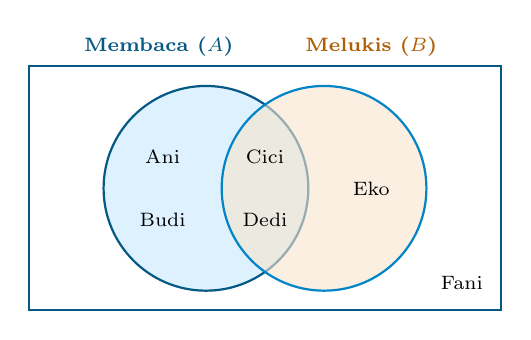
\begin{tikzpicture}
\draw[mainc,thick] (-3.0,-1.55) rectangle (3.0,1.55);
\draw[mainc,thick,fill=skyl!50] (-0.75,0) circle (1.3);
\draw[accc,thick,fill=warmc!20,fill opacity=0.6] (0.75,0) circle (1.3);
\node[font=\scriptsize\bfseries,mainc] at (-1.35,1.8) {Membaca ($A$)};
\node[font=\scriptsize\bfseries,warmc!80!black] at (1.35,1.8) {Melukis ($B$)};
\node[font=\scriptsize] at (-1.3,0.4) {Ani};
\node[font=\scriptsize] at (-1.3,-0.4) {Budi};
\node[font=\scriptsize] at (0,0.4) {Cici};
\node[font=\scriptsize] at (0,-0.4) {Dedi};
\node[font=\scriptsize] at (1.35,0) {Eko};
\node[font=\scriptsize] at (2.5,-1.2) {Fani};
\end{tikzpicture}}}{\pilx{Cici dan Dedi}{Eko}{Ani, Budi, dan Eko}{Ani, Budi, Cici, dan Dedi}{Ani dan Budi}}
\soal{Diketahui $P=\{x\mid x\text{ bilangan prima kurang dari }20\}$. Banyak anggota himpunan $P$ adalah \dots.}{\pil{$7$}{$8$}{$9$}{$10$}{$19$}}
\soal{\gbr{Diagram panah menunjukkan fungsi $f$ dari $A$ ke $B$. Daerah hasil fungsi $f$ adalah \dots.}{%
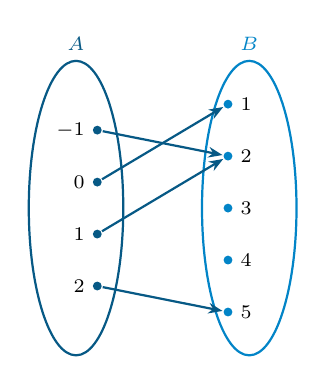
\begin{tikzpicture}
\sets{4}{$-1$,0,1,2}{5}{1,2,3,4,5}{$A$}{$B$}{2.2}{0.6}
\draw[ar,shorten >=2pt,shorten <=2pt] (a1)--(b2);
\draw[ar,shorten >=2pt,shorten <=2pt] (a2)--(b1);
\draw[ar,shorten >=2pt,shorten <=2pt] (a3)--(b2);
\draw[ar,shorten >=2pt,shorten <=2pt] (a4)--(b5);
\end{tikzpicture}}}{\pilx{$\{1,2,3,4,5\}$}{$\{-1,0,1,2\}$}{$\{1,2,2,5\}$}{$\{1,2,5\}$}{$\{2,5\}$}}
\soal{Diketahui $f(x)=3x-7$. Jika $f(a)=11$, maka nilai $f(a+2)$ adalah \dots.}{\pil{$13$}{$15$}{$17$}{$19$}{$23$}}

\tingkat{Tingkat Sedang}{soal 5 sampai 8}
\soal{Diketahui himpunan semesta $S=\{x\mid x\text{ bilangan asli},\ x\le12\}$, $A$ himpunan faktor dari $12$, dan $B$ himpunan kelipatan $3$ dalam $S$. Tentukan apakah tiap pernyataan berikut benar atau salah.\par\smallskip}{%
\begin{tabularx}{\linewidth}{@{}X>{\centering\arraybackslash}p{1.3cm}>{\centering\arraybackslash}p{1.3cm}@{}}
\hline \textbf{Pernyataan} & \textbf{Benar} & \textbf{Salah}\\ \hline
(1) $A\cap B=\{3,6,12\}$ & \kotak & \kotak\\
(2) $n(A\cup B)=10$ & \kotak & \kotak\\
(3) $A-B=\{1,2,4\}$ & \kotak & \kotak\\
(4) $n\big((A\cup B)^c\big)=6$ & \kotak & \kotak\\ \hline
\end{tabularx}}
\soal{\gbr{Diagram Cartesius menunjukkan relasi dari himpunan $A=\{1,2,3,4\}$ (sumbu mendatar) ke himpunan $B=\{2,4,6,8\}$ (sumbu tegak). Relasi yang tepat dari $A$ ke $B$ adalah \dots.}{%
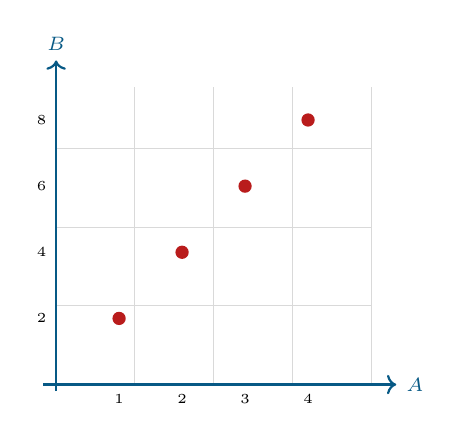
\begin{tikzpicture}[x=0.8cm,y=0.42cm]
\draw[gray!30] (0,0) grid (5,9);
\draw[->,thick,mainc] (-0.2,0)--(5.4,0) node[right,font=\scriptsize]{$A$};
\draw[->,thick,mainc] (0,-0.2)--(0,9.8) node[above,font=\scriptsize]{$B$};
\foreach \i in {1,2,3,4}{\node[font=\tiny,below] at (\i,0){$\i$};}
\foreach \j in {2,4,6,8}{\node[font=\tiny,left] at (0,\j){$\j$};}
\foreach \a/\b in {1/2,2/4,3/6,4/8}{\fill[brick] (\a,\b) circle (2.4pt);}
\end{tikzpicture}}}{\pilx{setengah dari}{dua kali dari}{faktor dari}{kurang dari}{kuadrat dari}}
\soal{Diketahui $A=\{1,2,3\}$ dan $B=\{p,q,r\}$. Empat relasi dari $A$ ke $B$ ditunjukkan oleh diagram panah berikut. Pilih \textbf{semua} diagram yang merupakan fungsi dari $A$ ke $B$.\par\smallskip}{%
\noindent\begin{minipage}{0.23\linewidth}\centering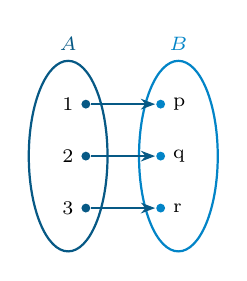
\begin{tikzpicture}
\sets{3}{1,2,3}{3}{p,q,r}{$A$}{$B$}{1.4}{0.5}
\draw[ar,shorten >=2pt,shorten <=2pt] (a1)--(b1);
\draw[ar,shorten >=2pt,shorten <=2pt] (a2)--(b2);
\draw[ar,shorten >=2pt,shorten <=2pt] (a3)--(b3);
\end{tikzpicture}\\[2pt]\kotak\ (1)\end{minipage}\hfill
\begin{minipage}{0.23\linewidth}\centering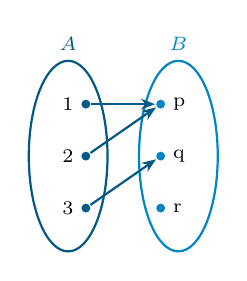
\begin{tikzpicture}
\sets{3}{1,2,3}{3}{p,q,r}{$A$}{$B$}{1.4}{0.5}
\draw[ar,shorten >=2pt,shorten <=2pt] (a1)--(b1);
\draw[ar,shorten >=2pt,shorten <=2pt] (a2)--(b1);
\draw[ar,shorten >=2pt,shorten <=2pt] (a3)--(b2);
\end{tikzpicture}\\[2pt]\kotak\ (2)\end{minipage}\hfill
\begin{minipage}{0.23\linewidth}\centering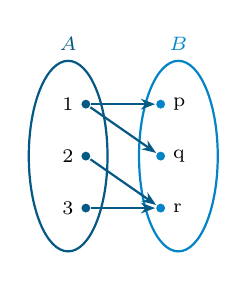
\begin{tikzpicture}
\sets{3}{1,2,3}{3}{p,q,r}{$A$}{$B$}{1.4}{0.5}
\draw[ar,shorten >=2pt,shorten <=2pt] (a1)--(b1);
\draw[ar,shorten >=2pt,shorten <=2pt] (a1)--(b2);
\draw[ar,shorten >=2pt,shorten <=2pt] (a2)--(b3);
\draw[ar,shorten >=2pt,shorten <=2pt] (a3)--(b3);
\end{tikzpicture}\\[2pt]\kotak\ (3)\end{minipage}\hfill
\begin{minipage}{0.23\linewidth}\centering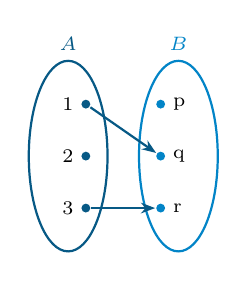
\begin{tikzpicture}
\sets{3}{1,2,3}{3}{p,q,r}{$A$}{$B$}{1.4}{0.5}
\draw[ar,shorten >=2pt,shorten <=2pt] (a1)--(b2);
\draw[ar,shorten >=2pt,shorten <=2pt] (a3)--(b3);
\end{tikzpicture}\\[2pt]\kotak\ (4)\end{minipage}}
\soal{\gbr{Grafik menunjukkan biaya mencetak foto, $c(n)$ dalam ribuan rupiah, untuk $n$ lembar di sebuah studio. Biaya terdiri atas biaya tetap dan biaya per lembar yang sama untuk semua lembar. Biaya mencetak $10$ lembar foto adalah \dots.}{%
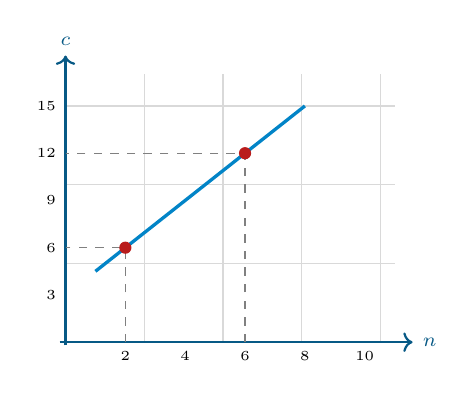
\begin{tikzpicture}[x=0.38cm,y=0.2cm]
\draw[gray!30] (0,0) grid (11,17);
\draw[->,thick,mainc] (-0.2,0)--(11.6,0) node[right,font=\scriptsize]{$n$};
\draw[->,thick,mainc] (0,-0.2)--(0,18.2) node[above,font=\scriptsize]{$c$};
\draw[accc,very thick] (1,4.5)--(8,15);
\draw[dashed,gray] (2,0)--(2,6)--(0,6);
\draw[dashed,gray] (6,0)--(6,12)--(0,12);
\fill[brick] (2,6) circle (2.2pt) (6,12) circle (2.2pt);
\foreach \i in {2,4,6,8,10}{\node[font=\tiny,below] at (\i,0){$\i$};}
\foreach \j in {3,6,9,12,15}{\node[font=\tiny,left] at (0,\j){$\j$};}
\end{tikzpicture}}}{\pil{Rp15.000}{Rp16.500}{Rp18.000}{Rp20.000}{Rp30.000}}

\tingkat{Tingkat Sulit}{soal 9 sampai 11}
\soal{\gbr{Dari $37$ siswa kelas 8, sebanyak $25$ siswa mengikuti Pramuka ($P$), $18$ siswa mengikuti Robotik ($R$), dan banyak siswa yang mengikuti \textbf{kedua} kegiatan sama dengan tiga kali banyak siswa yang \textbf{tidak mengikuti keduanya}. Diagram Venn memakai $x$ untuk banyak siswa yang tidak mengikuti keduanya. Banyak siswa yang mengikuti tepat satu kegiatan adalah \dots.}{%
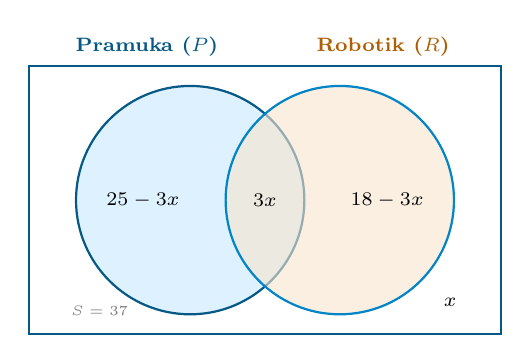
\begin{tikzpicture}
\draw[mainc,thick] (-3.0,-1.7) rectangle (3.0,1.7);
\draw[mainc,thick,fill=skyl!50] (-0.95,0) circle (1.45);
\draw[accc,thick,fill=warmc!20,fill opacity=0.6] (0.95,0) circle (1.45);
\node[font=\scriptsize\bfseries,mainc] at (-1.5,1.95) {Pramuka ($P$)};
\node[font=\scriptsize\bfseries,warmc!80!black] at (1.5,1.95) {Robotik ($R$)};
\node[font=\scriptsize] at (-1.55,0) {$25-3x$};
\node[font=\scriptsize] at (0,0) {$3x$};
\node[font=\scriptsize] at (1.55,0) {$18-3x$};
\node[font=\scriptsize] at (2.35,-1.3) {$x$};
\node[font=\tiny,gray] at (-2.1,-1.4) {$S=37$};
\end{tikzpicture}}}{\pil{$3$}{$9$}{$16$}{$25$}{$34$}}
\soal{Fungsi $f(x)=ax+b$ dengan $a\ne0$ memiliki daerah asal $\{1,2,3\}$ dan daerah hasil $\{4,10,16\}$. Nilai $f(0)$ yang mungkin adalah \dots.}{\pil{$-2$ saja}{$4$ atau $16$}{$10$}{$22$ saja}{$-2$ atau $22$}}
\soal{Diketahui $K=\{x\mid x\text{ bilangan asli},\ x^2<50\}$. Banyak himpunan bagian \textbf{tak kosong} dari $K$ yang semua anggotanya bilangan ganjil adalah \dots.}{\pil{$15$}{$16$}{$31$}{$64$}{$127$}}

\Needspace{16\baselineskip}
\tingkat{Tingkat HOTS}{soal 12, penalaran tingkat tinggi}
\soal{\gbr{Empat siswa (Ayu, Beni, Citra, Dodi) masing-masing memilih \textbf{tepat satu} dari tiga klub (Catur, Teater, Lukis). Misalkan $f$ menyatakan klub yang dipilih tiap siswa. Gambar menunjukkan \textbf{satu} kemungkinan hasil pemilihan. Pilih \textbf{semua} pernyataan yang benar tentang pemilihan klub tersebut (untuk semua kemungkinan hasil pemilihan).}{%
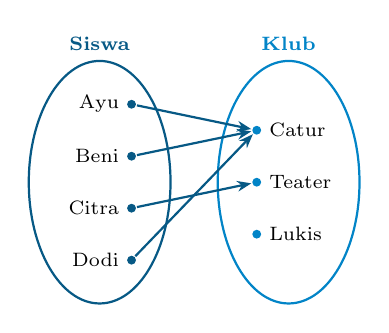
\begin{tikzpicture}
\sets{4}{Ayu,Beni,Citra,Dodi}{3}{Catur,Teater,Lukis}{Siswa}{Klub}{2.4}{0.9}
\draw[ar,shorten >=2pt,shorten <=2pt] (a1)--(b1);
\draw[ar,shorten >=2pt,shorten <=2pt] (a2)--(b1);
\draw[ar,shorten >=2pt,shorten <=2pt] (a3)--(b2);
\draw[ar,shorten >=2pt,shorten <=2pt] (a4)--(b1);
\end{tikzpicture}}}{%
\begin{tabularx}{\linewidth}{@{}lX@{}}
\kotak & (1) Pemilihan klub tersebut selalu merupakan fungsi dari siswa ke klub.\\
\kotak & (2) Pemilihan klub tersebut dapat berupa fungsi injektif.\\
\kotak & (3) Pemilihan klub tersebut dapat berupa fungsi surjektif.\\
\kotak & (4) Jika Ayu dan Beni memilih klub yang sama, maka $f$ tidak mungkin surjektif.\\
\kotak & (5) Jika $f$ surjektif, maka ada tepat satu klub yang dipilih oleh dua siswa.
\end{tabularx}}

% =====================================================================
\Needspace{14\baselineskip}
\bagian{B. Isian Singkat}{5 soal $\times$ 4 poin = 20 poin. Tuliskan hanya jawaban akhir.}

\tingkat{Tingkat Sedang}{soal 1 dan 2}
\soal{Diketahui $P=\{x\mid x\text{ bilangan ganjil},\ 2<x<14\}$ dan $Q=\{x\mid x\text{ bilangan asli kelipatan }3,\ x<16\}$. Nilai $n(P\cup Q)$ adalah \dots.}{\jwb}
\soal{Fungsi $f(x)=x^2-3x$ memiliki daerah asal $\{0,1,2,3\}$. Banyak anggota daerah hasil $f$ adalah \dots.}{\jwb}

\tingkat{Tingkat Sulit}{soal 3 sampai 5}
\soal{Di sebuah kelas terdapat $40$ siswa. Sebanyak $28$ siswa gemar sepak bola dan $25$ siswa gemar voli. Tidak diketahui apakah ada siswa yang tidak gemar keduanya. Selisih antara nilai \textbf{terbesar} dan nilai \textbf{terkecil} yang mungkin bagi banyak siswa yang gemar keduanya adalah \dots.}{\jwb}
\soal{Pada $A=\{1,2,3,\dots,10\}$ didefinisikan relasi $R$ dari $A$ ke $A$: $(a,b)\in R$ jika $a$ faktor dari $b$ dan $a<b$. Banyak pasangan berurutan dalam $R$ adalah \dots.}{\jwb}
\soal{\gbr{Sebuah mesin mengubah bilangan masukan $x$ menjadi keluaran $f(x)$ dengan aturan $f(x)=ax^2+b$ (lihat tabel). Nilai $f(7)$ adalah \dots.}{%
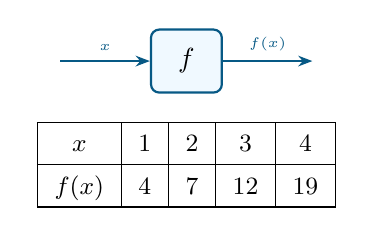
\begin{tikzpicture}
\node[box,minimum width=0.9cm,minimum height=0.8cm] (m) at (0,0) {$f$};
\draw[ar] (-1.6,0)--(m) node[midway,above,font=\tiny]{$x$};
\draw[ar] (m)--(1.6,0) node[midway,above,font=\tiny]{$f(x)$};
\node[font=\small,below=0.15cm] at (0,-0.5) {%
\begin{tabular}{|c|c|c|c|c|}\hline $x$ & $1$ & $2$ & $3$ & $4$\\ \hline $f(x)$ & $4$ & $7$ & $12$ & $19$\\ \hline\end{tabular}};
\end{tikzpicture}}}{\jwb}

% =====================================================================
\Needspace{16\baselineskip}
\bagian{C. Uraian (Essay)}{3 soal: 12 + 14 + 18 = 44 poin. Tuliskan langkah penyelesaian dengan lengkap.}

\tingkat{Tingkat Sedang}{soal 1}
\soal{\gbr{Empat siswa, yaitu Ali, Bima, Citra, dan Dina, mendaftar ekstrakurikuler. Relasi ``mengikuti'' dari himpunan siswa ke himpunan ekstrakurikuler $\{$Pramuka, Futsal, Musik$\}$ ditunjukkan pada diagram panah.\par\smallskip
(a) Tuliskan relasi tersebut sebagai himpunan pasangan berurutan dan tentukan banyak pasangannya.\par
(b) Apakah relasi tersebut fungsi dari siswa ke ekstrakurikuler? Jelaskan, dan sebutkan siswa yang menyebabkannya.\par
(c) Sekolah mewajibkan tiap siswa hanya boleh mengikuti satu ekstrakurikuler. Berapa pasangan paling sedikit yang harus dihapus agar relasi menjadi fungsi, dan ada berapa cara menghapusnya?\par
(d) Dari semua cara pada (c), berapa yang menghasilkan fungsi surjektif ke $\{$Pramuka, Futsal, Musik$\}$? Apakah ada yang injektif? Jelaskan.}{%
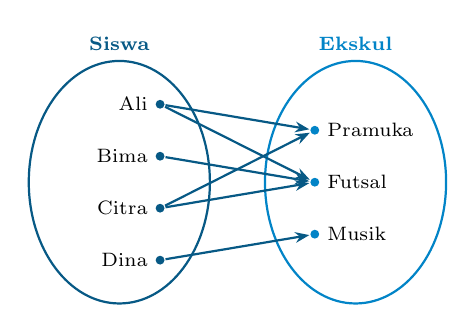
\begin{tikzpicture}
\sets{4}{Ali,Bima,Citra,Dina}{3}{Pramuka,Futsal,Musik}{Siswa}{Ekskul}{3.0}{1.15}
\draw[ar,shorten >=2pt,shorten <=2pt] (a1)--(b1);
\draw[ar,shorten >=2pt,shorten <=2pt] (a1)--(b2);
\draw[ar,shorten >=2pt,shorten <=2pt] (a2)--(b2);
\draw[ar,shorten >=2pt,shorten <=2pt] (a3)--(b1);
\draw[ar,shorten >=2pt,shorten <=2pt] (a3)--(b2);
\draw[ar,shorten >=2pt,shorten <=2pt] (a4)--(b3);
\end{tikzpicture}}}{\poin{12}}

\Needspace{22\baselineskip}
\tingkat{Tingkat Sulit}{soal 2}
\soal{\gbr{Dua lilin dinyalakan bersamaan. Lilin $A$ mula-mula setinggi $30$ cm dan setelah $10$ jam tersisa $10$ cm. Lilin $B$ mula-mula setinggi $24$ cm dan setelah $4$ jam tersisa $18$ cm. Kedua lilin terbakar dengan laju tetap (lihat grafik). Misalkan $A(t)$ dan $B(t)$ adalah tinggi lilin (cm) setelah $t$ jam.\par\smallskip
(a) Tentukan rumus $A(t)$ dan $B(t)$.\par
(b) Setelah $8$ jam, lilin mana yang lebih tinggi dan berapa selisihnya?\par
(c) Setelah berapa jam kedua lilin sama tinggi, dan berapa tinggi mereka?\par
(d) Lilin $A$ habis terbakar setelah berapa jam? Pada saat itu, berapa tinggi lilin $B$? Tuliskan daerah asal fungsi $A$ yang masuk akal.}{%
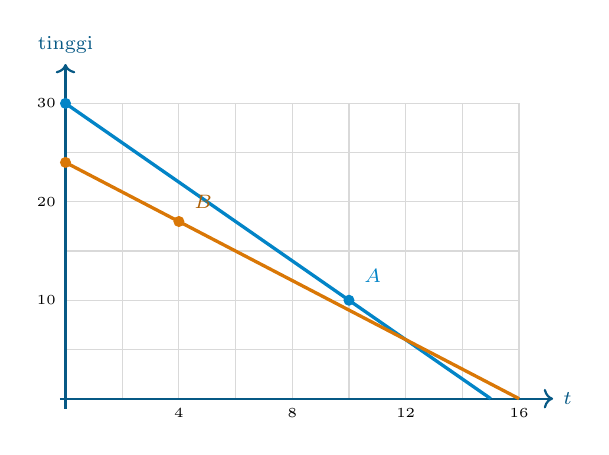
\begin{tikzpicture}[x=0.36cm,y=0.125cm]
\draw[gray!30] (0,0) grid[xstep=2,ystep=5] (16,30);
\draw[->,thick,mainc] (-0.2,0)--(17.2,0) node[right,font=\scriptsize]{$t$};
\draw[->,thick,mainc] (0,-1)--(0,34) node[above,font=\scriptsize]{tinggi};
\draw[accc,very thick] (0,30)--(15,0);
\draw[warmc,very thick] (0,24)--(16,0);
\fill[accc] (0,30) circle (2pt) (10,10) circle (2pt);
\fill[warmc] (0,24) circle (2pt) (4,18) circle (2pt);
\node[font=\scriptsize,accc,right] at (10.2,12.5) {$A$};
\node[font=\scriptsize,warmc!80!black,right] at (4.2,20) {$B$};
\foreach \i in {4,8,12,16}{\node[font=\tiny,below] at (\i,0){$\i$};}
\foreach \j in {10,20,30}{\node[font=\tiny,left] at (0,\j){$\j$};}
\end{tikzpicture}}}{\poin{14}}

\Needspace{15\baselineskip}
\tingkat{Tingkat HOTS}{soal 3}
\soal{\gbr{Tiga siswa $X$, $Y$, dan $Z$ akan duduk pada empat kursi bernomor $1,2,3,4$. Setiap siswa menempati tepat satu kursi dan \textbf{tidak ada dua siswa yang menempati kursi yang sama}. Gambar menunjukkan salah satu penempatan.\par\smallskip
(a) Jelaskan mengapa penempatan pada gambar merupakan fungsi injektif tetapi bukan fungsi surjektif.\par
(b) Tentukan banyak semua penempatan yang mungkin dan jelaskan cara menghitungnya.\par
(c) Tentukan banyak penempatan jika $X$ dan $Y$ harus duduk pada dua kursi yang nomornya berurutan.\par
(d) Pada kasus lain, terdapat $4$ siswa dan $4$ kursi. Dina berpendapat, ``Jika tidak ada dua siswa yang menempati kursi yang sama, maka pasti semua kursi terisi.'' Benarkah pendapat Dina? Berikan alasan, lalu tentukan banyak penempatan pada kasus ini.}{%
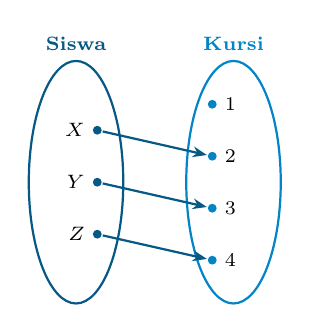
\begin{tikzpicture}
\sets{3}{$X$,$Y$,$Z$}{4}{1,2,3,4}{Siswa}{Kursi}{2.0}{0.6}
\draw[ar,shorten >=2pt,shorten <=2pt] (a1)--(b2);
\draw[ar,shorten >=2pt,shorten <=2pt] (a2)--(b3);
\draw[ar,shorten >=2pt,shorten <=2pt] (a3)--(b4);
\end{tikzpicture}}}{\poin{18}}

% =====================================================================
\newpage
\bagian{Kunci Jawaban dan Pembahasan Singkat}{Untuk guru dan pembahasan mandiri}
\par\vspace{0.6em}{\bfseries\color{mainc}Kunci Pilihan Ganda}\par\vspace{0.3em}
\small
\begin{tabularx}{\linewidth}{@{}*{6}{>{\centering\arraybackslash}X}@{}}\hline \textbf{1} & \textbf{2} & \textbf{3} & \textbf{4} & \textbf{5} & \textbf{6}\\ \hline E & B & D & C & B, S, B, S & A\\ \hline\end{tabularx}\\[6pt]
\begin{tabularx}{\linewidth}{@{}*{6}{>{\centering\arraybackslash}X}@{}}\hline \textbf{7} & \textbf{8} & \textbf{9} & \textbf{10} & \textbf{11} & \textbf{12}\\ \hline (1) dan (2) & C & D & E & A & (1), (3), (5)\\ \hline\end{tabularx}
\par\vspace{0.4em}{\bfseries\color{mainc}Kunci Isian Singkat:}\ \ 1) $9$\quad 2) $2$\quad 3) $12$\quad 4) $17$\quad 5) $52$
\par\vspace{0.8em}{\bfseries\color{mainc}\normalsize Pembahasan Pilihan Ganda}\par\vspace{0.2em}
\small\begin{enumerate}[leftmargin=2em,itemsep=2pt,topsep=2pt]
\item[\textbf{1.}] \textbf{(E)} $A-B$ berisi anggota $A$ yang tidak berada di irisan: Ani dan Budi. (Jebakan: Cici dan Dedi adalah $A\cap B$, sedangkan Eko adalah $B-A$.)
\item[\textbf{2.}] \textbf{(B)} $P=\{2,3,5,7,11,13,17,19\}$, sehingga $n(P)=8$. (Jebakan: $1$ bukan bilangan prima sehingga menghasilkan $9$; atau $2$ dikira bukan prima sehingga menghasilkan $7$.)
\item[\textbf{3.}] \textbf{(D)} Daerah hasil adalah anggota $B$ yang mendapat pasangan: $-1\to2$, $0\to1$, $1\to2$, $2\to5$. Anggota yang sama ditulis sekali, jadi $\{1,2,5\}$. Anggota $3$ dan $4$ tidak mendapat pasangan. (Jebakan: memilih daerah asal, daerah kawan, atau menulis $2$ dua kali.)
\item[\textbf{4.}] \textbf{(C)} $3a-7=11$ sehingga $a=6$ dan $f(8)=24-7=17$. Cara cepat: menambah $2$ pada $x$ menambah $3\cdot2=6$ pada $f(x)$, jadi $11+6=17$. (Jebakan: $11+2=13$.)
\item[\textbf{5.}] \textbf{(B, S, B, S)} $A=\{1,2,3,4,6,12\}$ dan $B=\{3,6,9,12\}$. (1) $A\cap B=\{3,6,12\}$: benar. (2) $A\cup B=\{1,2,3,4,6,9,12\}$ sehingga $n=7$, bukan $10$; nilai $10=n(A)+n(B)$ menghitung ganda $3,6,12$: salah. (3) $A-B=\{1,2,4\}$: benar. (4) $(A\cup B)^c=\{5,7,8,10,11\}$ berisi $5$ anggota, bukan $6$: salah.
\item[\textbf{6.}] \textbf{(A)} Pasangannya $(1,2),(2,4),(3,6),(4,8)$ dibaca ``$1$ setengah dari $2$'', dan seterusnya. ``Dua kali dari'' adalah arah sebaliknya (dari $B$ ke $A$). ``Faktor dari'' akan menghasilkan lebih banyak pasangan, misalnya $(1,4)$, $(1,6)$, $(1,8)$, $(2,6)$, $(2,8)$ yang tidak ada pada gambar.
\item[\textbf{7.}] \textbf{(1) dan (2)} Fungsi menuntut setiap anggota $A$ memiliki \emph{tepat satu} panah. (1) ya (bahkan bijektif). (2) ya, karena $1$ dan $2$ boleh berbagi pasangan $p$. (3) bukan, karena $1$ memiliki dua panah. (4) bukan, karena $2$ tidak memiliki panah.
\item[\textbf{8.}] \textbf{(C)} Dari titik $(2;6)$ dan $(6;12)$ (ribuan rupiah), biaya per lembar $=\frac{12-6}{6-2}=1{,}5$ ribu, yaitu Rp1.500. Biaya tetap $=6.000-2\cdot1.500=3.000$. Jadi $c(n)=1.500n+3.000$ dan $c(10)=18.000$. (Jebakan: Rp30.000 bila grafik dianggap melalui titik asal, dan Rp15.000 atau Rp16.500 bila salah menghitung lembar.)
\item[\textbf{9.}] \textbf{(D)} Jumlah semua daerah pada diagram: $(25-3x)+3x+(18-3x)+x=43-2x=37$, sehingga $x=3$. Tepat satu kegiatan: $(25-9)+(18-9)=16+9=25$. (Jebakan: $34$ adalah yang mengikuti paling sedikit satu kegiatan, $9$ adalah yang mengikuti keduanya, dan $3$ adalah yang tidak mengikuti keduanya.)
\item[\textbf{10.}] \textbf{(E)} Karena $a\ne0$, fungsi linear naik terus atau turun terus. Ketiga nilai $4,10,16$ berselisih $6$. Jika $a>0$: $f(1)=4$, $f(2)=10$, $f(3)=16$ sehingga $a=6$, $b=-2$ dan $f(0)=-2$. Jika $a<0$: $f(1)=16$, $f(2)=10$, $f(3)=4$ sehingga $a=-6$, $b=22$ dan $f(0)=22$. Keduanya memenuhi, jadi $f(0)=-2$ atau $22$. (Jebakan: hanya memikirkan $a$ positif.)
\item[\textbf{11.}] \textbf{(A)} $K=\{1,2,3,4,5,6,7\}$ karena $7^2=49<50$ dan $8^2=64>50$. Anggota ganjil: $\{1,3,5,7\}$ ($4$ anggota) dengan $2^4=16$ himpunan bagian, termasuk himpunan kosong. Tak kosong: $16-1=15$. (Jebakan: $16$ bila himpunan kosong ikut dihitung, dan $127$ yaitu himpunan bagian tak kosong dari seluruh $K$.)
\item[\textbf{12.}] \textbf{(1), (3), dan (5)} (1) benar: tiap siswa memilih tepat satu klub. (2) salah: $4$ siswa dan $3$ klub, jadi pasti ada dua siswa yang sama klub, sehingga tidak mungkin injektif. (3) benar: misalnya Ayu dan Beni Catur, Citra Teater, Dodi Lukis; semua klub terpilih. (4) salah: contoh pada (3) memiliki Ayu dan Beni di klub yang sama tetapi tetap surjektif. (5) benar: surjektif berarti tiap klub dipilih minimal satu siswa; dengan $4$ siswa, pembagiannya haruslah $2+1+1$, sehingga tepat satu klub berisi dua siswa.
\end{enumerate}
\par\Needspace{6\baselineskip}\vspace{0.6em}{\bfseries\color{mainc}\normalsize Pembahasan Isian Singkat}\par\vspace{0.2em}
\small\begin{enumerate}[leftmargin=2em,itemsep=2pt,topsep=2pt]
\item[\textbf{1.}] \textbf{Jawaban: $9$.} $P=\{3,5,7,9,11,13\}$ ($6$ anggota) dan $Q=\{3,6,9,12,15\}$ ($5$ anggota). Irisan $P\cap Q=\{3,9\}$ ($2$ anggota; $15$ tidak termasuk karena $15\not<14$). $n(P\cup Q)=6+5-2=9$.
\item[\textbf{2.}] \textbf{Jawaban: $2$.} $f(0)=0$, $f(1)=-2$, $f(2)=-2$, $f(3)=0$. Daerah hasil $\{0,-2\}$ hanya memiliki $2$ anggota, walaupun daerah asalnya $4$ anggota (fungsi ini tidak injektif).
\item[\textbf{3.}] \textbf{Jawaban: $12$.} Misalkan $U$ banyak siswa yang gemar paling sedikit satu olahraga. Maka $n(\text{keduanya})=28+25-U=53-U$. $U$ paling kecil $28$ (semua penggemar voli juga penggemar sepak bola) dan paling besar $40$ (semua siswa). Jadi nilai terbesar $=53-28=25$ dan nilai terkecil $=53-40=13$. Selisih $25-13=12$.
\item[\textbf{4.}] \textbf{Jawaban: $17$.} Hitung per nilai $a$: $a=1$ ada $9$ pasangan ($b=2,\dots,10$); $a=2$: $b=4,6,8,10$ ($4$); $a=3$: $b=6,9$ ($2$); $a=4$: $b=8$ ($1$); $a=5$: $b=10$ ($1$). Total $9+4+2+1+1=17$.
\item[\textbf{5.}] \textbf{Jawaban: $52$.} Dari $f(1)=a+b=4$ dan $f(2)=4a+b=7$ diperoleh $a=1$ dan $b=3$, jadi $f(x)=x^2+3$. Cek: $f(3)=12$ dan $f(4)=19$. Maka $f(7)=49+3=52$.
\end{enumerate}
\par\Needspace{8\baselineskip}\vspace{0.6em}{\bfseries\color{mainc}\normalsize Pembahasan dan Pedoman Penskoran Uraian}\par\vspace{0.2em}
\small\begin{enumerate}[leftmargin=2em,itemsep=3pt,topsep=2pt]
\item[\textbf{1.}] (a) $R=\{(\text{Ali},\text{Pramuka}),$ $(\text{Ali},\text{Futsal}),$ $(\text{Bima},\text{Futsal}),$ $(\text{Citra},\text{Pramuka}),$ $(\text{Citra},\text{Futsal}),$ $(\text{Dina},\text{Musik})\}$, banyaknya $6$ pasangan. (b) Bukan fungsi, karena fungsi menuntut setiap siswa dipasangkan dengan \emph{tepat satu} ekstrakurikuler, sedangkan Ali dan Citra masing-masing memiliki dua pasangan. (c) Ali harus memilih satu dari dua pasangannya (hapus $1$) dan Citra juga (hapus $1$); Bima dan Dina sudah tepat satu pasangan. Pasangan yang dihapus paling sedikit adalah $2$, dengan banyak cara $2\times2=4$. (d) Bima selalu Futsal dan Dina selalu Musik, sehingga Futsal dan Musik pasti punya anggota. Agar Pramuka punya anggota, Ali atau Citra harus memilih Pramuka. Satu-satunya cara yang gagal adalah keduanya memilih Futsal, jadi surjektif ada $4-1=3$ cara. Tidak ada yang injektif karena $4$ siswa hanya dipasangkan ke $3$ ekstrakurikuler, sehingga pasti ada yang berbagi pasangan. \\ \textit{Penskoran: tiap bagian 3 poin.}
\item[\textbf{2.}] (a) Laju lilin $A$: $\frac{30-10}{10}=2$ cm/jam, jadi $A(t)=30-2t$. Laju lilin $B$: $\frac{24-18}{4}=1{,}5$ cm/jam, jadi $B(t)=24-1{,}5t$. (b) $A(8)=30-16=14$ cm dan $B(8)=24-12=12$ cm. Lilin $A$ lebih tinggi $2$ cm. (c) Sama tinggi: $30-2t=24-1{,}5t\Rightarrow6=0{,}5t\Rightarrow t=12$ jam, dan tingginya $30-24=6$ cm (cek: $24-18=6$). (d) $A(t)=0\Rightarrow t=15$ jam. Pada saat itu $B(15)=24-22{,}5=1{,}5$ cm. Daerah asal yang masuk akal untuk $A$ adalah semua $t$ dengan $0\le t\le15$ (waktu tidak negatif dan lilin sudah habis setelah $15$ jam). \\ \textit{Penskoran: (a) 3 poin; (b) 3 poin; (c) 4 poin; (d) 4 poin.}
\item[\textbf{3.}] (a) Pada gambar $X\to2$, $Y\to3$, $Z\to4$. Tiap siswa mendapat tepat satu kursi (fungsi) dan tidak ada dua siswa yang berbagi kursi, jadi injektif. Daerah hasil $\{2,3,4\}$ tidak sama dengan daerah kawan $\{1,2,3,4\}$ karena kursi $1$ tidak mendapat pasangan, jadi tidak surjektif. (b) $X$ memiliki $4$ pilihan kursi, $Y$ memiliki $3$ pilihan (kursi $X$ tidak boleh dipakai), $Z$ memiliki $2$ pilihan. Banyaknya $4\times3\times2=24$ penempatan. (c) Pasangan kursi $(X,Y)$ yang berurutan: $(1,2),(2,1),(2,3),(3,2),(3,4),(4,3)$, yaitu $6$. Untuk tiap pasangan, $Z$ dapat menempati $2$ kursi sisa. Banyaknya $6\times2=12$. (d) Pendapat Dina benar. Jika $4$ siswa menempati $4$ kursi yang semuanya berbeda, maka kursi yang terpakai ada $4$; karena hanya ada $4$ kursi, semua kursi terisi (fungsi menjadi surjektif, jadi bijektif). Banyak penempatan: $4\times3\times2\times1=24$. \\ \textit{Penskoran: (a) 3 poin; (b) 4 poin; (c) 5 poin; (d) 6 poin.}
\end{enumerate}
\end{document}
